\part{Session 1}

\section{mbed Environment}
\subsection{What is mbed}
\begin{frame}
	\frametitle{What is mbed?}
	The mbed system provides:
	\begin{itemize}
		\item \textbf{Free} software libraries
		\item \textbf{Free} hardware designs
		\item \textbf{Free} online development tools
		\item Developer community
	\end{itemize}
	\begin{block}{What this means}
		Shorter development, lower cost
	\end{block}
\end{frame}

\begin{frame}
	\frametitle{Software Development Kit}
	\begin{itemize}
		\item Open source C/C++ libraries\\
			Safe for personal or commercial use
		\item Hardware abstraction layer\\
			Isolate your application code from hardware changes
		\item Built from CMSIS APIs\\
			Work with high level functions or bare metal hardware
		\item Pretested startup and peripheral libraries
	\end{itemize}
\end{frame}

\begin{frame}
	\frametitle{Hardware Development Kit}
	The mbed Hardware Development Kit provides ready to use boards like the Nucleo as well as open source tools to develop custom boards.
	\begin{itemize}
		\item CMSIS-DAP based USB drag-n-drop programmer and debugger
		\item Virtual serial port
	\end{itemize}
\end{frame}

\begin{frame}[t]
	\frametitle{Online Development Tools}
	\begin{columns}[T]
		\begin{column}{0.5\textwidth}
			\begin{itemize}
				\item Professional ARM C/C++ compiler with optimization
				\item Cloud based IDE that allows you to work from anywhere
				\item Tightly integrated with a Mercurial based version control system
				\item Search, import, and publish open source libraries
				\item Export to several offline toolchains
			\end{itemize}
		\end{column}
		\begin{column}{0.5\textwidth}
			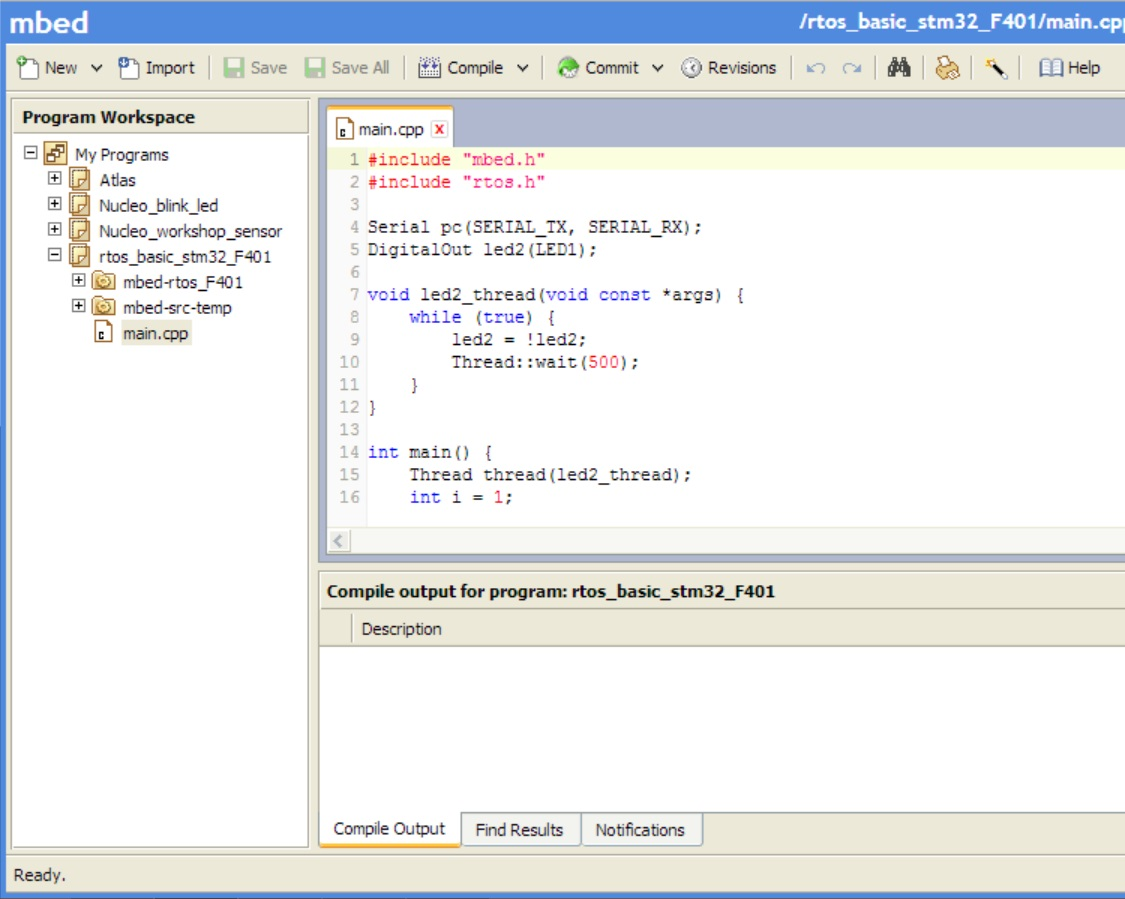
\includegraphics[width=\linewidth]{compiler}
		\end{column}
	\end{columns}
\end{frame}

\subsection{Nucleo Platform}
\begin{frame}
	\frametitle{Nucleo F401RE}
	\begin{columns}[T]
		\begin{column}{0.5\textwidth}
			The Nucleo platform combines a programmer/debugger and an STM32 based development board with Arduino compatible expansion headers.
			\begin{itemize}
				\item Up to 84 MHz clock speed
				\item 512 KBytes flash memory
				\item 12-bit 2.4 Msps ADC with up to 10 channels
				\item Three hardware USART
				\item Three hardware SPI
				\item Three hardware I2C
			\end{itemize}
		\end{column}
		\begin{column}{0.5\textwidth}
			%XXX center vertically
			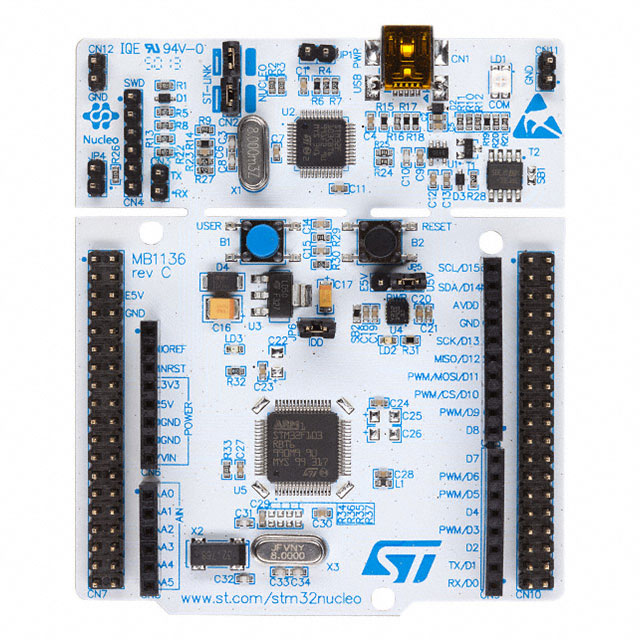
\includegraphics[width=\linewidth]{nucleo}
		\end{column}
	\end{columns}
\end{frame}

\section{Software Overview}

\section{Hardware Overview}
\subsection{Atlas Data Logger}
\begin{frame}
	\frametitle{Atlas Data Logger}
\end{frame}

\subsection{ADC: Analog to Digital Converter}
\begin{frame}
	\frametitle{ADC Overview}
\end{frame}

\subsection{USART: Universal Asynchronous Receiver/Transmitter}
\begin{frame}
	\frametitle{USART Overview}
\end{frame}

\subsection{SPI: Serial Peripheral Interface}
\begin{frame}
	\frametitle{SPI Overview}
\end{frame}

\subsection{I2C: Inter-Integrated Circuit}
\begin{frame}
	\frametitle{I2C Overview}
\end{frame}

\section{Resources}
\begin{frame}
	\frametitle{Online Resources}
\end{frame}